% === PRL Letter (edited) — Gauge‑Aligned Graviton Emergence (GAGE)
% Edits marked with `% CHANGE:` or `% MOVE:`

\pdfoutput=1
\documentclass[aps,prl,twocolumn,showpacs,superscriptaddress,nofootinbib,reprint]{revtex4-2}
\usepackage{amsmath,amssymb,amsfonts,mathtools}
\usepackage{array}
\usepackage{graphicx}
\usepackage{physics}
\usepackage{siunitx}
\AtBeginDocument{\RenewCommandCopy\qty\SI}
\usepackage[hidelinks]{hyperref}
\usepackage[nameinlink,capitalise]{cleveref}
\usepackage{microtype}
\usepackage{xspace}
\usepackage{bm}
\sisetup{separate-uncertainty=true}
\allowdisplaybreaks
\usepackage{tikz}
\usepackage{pgfplots} \pgfplotsset{compat=1.18}
\usetikzlibrary{positioning}

% avoid conflicts with physics/amsmath
\let\dd\relax\let\abs\relax\let\norm\relax\let\braket\relax\let\vev\relax\let\tr\relax\let\order\relax

% ==============================
% GAGE Macros (MS-bar@MZ default)
% ==============================

% ------- Global toggles -------
\newif\ifPRLBoxes   \PRLBoxestrue
\newif\ifUseSI      \UseSIfalse     % default: natural/Planck units (\Omega_\chi = G_N m_p^2)
\newcommand{\maybeBox}[1]{\ifPRLBoxes\boxed{#1}\else#1\fi}

% ---------- Constants ----------
\providecommand{\GN}{G_{\mathrm N}}
\providecommand{\MPl}{M_{\rm P}}            % reduced Planck mass
\providecommand{\Mp}{m_p}
\providecommand{\hbarc}{\hbar c}

% ---------- Scales ----------
\providecommand{\MZ}{M_Z}
\providecommand{\Mstar}{M_\ast}

% ---------- Gauge couplings (hats = MS-bar@MZ) ----------
\providecommand{\alphas}{\hat{\alpha}_s}
\providecommand{\alphaTwo}{\hat{\alpha}_2}
\providecommand{\alphae}{\hat{\alpha}}
\providecommand{\alphaGpp}{\alpha^{(\mathrm{pp})}_{G}}

% ---------- Integer projection / depth ----------
\providecommand{\chis}{\boldsymbol{\chi}}         % (16,13,2)
\providecommand{\Psivec}{\hat{\boldsymbol{\Psi}}} % (ln hats)
\providecommand{\XiDepth}{\hat{\Xi}}              % \hat\Xi = \chi·\hat\Psi
\providecommand{\XiEq}{\hat{\Xi}^{(\mathrm{eq})}}
\providecommand{\DXi}{\Delta\hat{\Xi}}

% ---------- Gate ----------
\DeclareRobustCommand{\PiGate}[1]{\Pi\!\left(#1\right)}
\providecommand{\sigchi}{\sigma_{\chi}}
\providecommand{\Gstar}{G_\ast}                   % equilibrium coupling (SM-only)
\providecommand{\Gx}{\Gstar\,\PiGate{\XiDepth}}
\let\Gate\PiGate

% ---------- Field-space metric ----------
\providecommand{\Kfs}{\mathbf{K}(\Psivec)}
\providecommand{\Keq}{\mathbf{K}_{\rm eq}}
\DeclareRobustCommand{\normK}[1]{\ensuremath{\left\lVert#1\right\rVert_{\Keq}}}

% ---------- Derived canonicals ----------
\providecommand{\Lgate}{\Lambda_{\mathrm{gate}}}

% ---------- Math utils ----------
\providecommand{\LN}{\ln}
\providecommand{\dd}{\mathrm{d}}
\providecommand{\vev}{\langle\,\cdot\,\rangle}
\DeclareMathOperator{\tr}{tr}
\providecommand{\abs}[1]{\ensuremath{\lvert#1\rvert}}
\providecommand{\norm}[1]{\ensuremath{\lVert#1\rVert}}
\providecommand{\order}[1]{\ensuremath{\mathcal{O}(#1)}}
\providecommand{\MSbar}{\overline{\mathrm{MS}}}

% ---------- GAGE invariant ----------
\providecommand{\OmegaChi}{\Omega_{\chis}}        % = alpha_s^16 alpha_2^13 alpha^2

% ---------- Display boxes ----------
\providecommand{\OmegaChiProdBox}{\maybeBox{\Omega_{\chis} \;=\; \alphas^{16}\,\alphaTwo^{13}\,\alphae^{2}}}
\providecommand{\GageLawBoxNat}{\maybeBox{\Omega_{\chis} \;=\; \GN\,\Mp^{2}}}
\providecommand{\GageLawBoxSI}{\maybeBox{\Omega_{\chis} \;=\; \GN\,\Mp^{2} / \hbarc}}
\providecommand{\GageLawBox}{\ifUseSI\GageLawBoxSI\else\GageLawBoxNat\fi}

% ---------- Lichnerowicz ----------
\providecommand{\DeltaL}{\Delta_{\!L}}

% ---------- Canonical \u0394G/G ----------
\providecommand{\FracDG}{\frac{\Delta G}{G}}

% ---------- Gate + lab-null boxes ----------
\providecommand{\GateBox}{\maybeBox{\frac{\Gx}{\Gstar} \;=\; \PiGate{\XiDepth}
\;=\; \exp\!\Big[-\frac{(\XiDepth-\XiEq)^2}{\sigchi^2}\Big]}}
\providecommand{\ParityNullBox}{\maybeBox{\FracDG\;\simeq\;\frac{\DXi^2}{\sigchi^2}
\quad(\Pi'(\XiEq)=0,\; G(x)=\Gstar\,\Pi(\Xi))}}

% ---------- Equilibrium emergent coupling ----------
\providecommand{\G}{G}
\providecommand{\GEquilBox}{\maybeBox{ \G \;=\; \frac{\hbarc}{\Mp^{2}}\,\OmegaChi }}

% ---------- Soft-mode scalar ----------
\providecommand{\phiChi}{\phi_{\chis}}
\providecommand{\ParityNullPhiBox}{\maybeBox{\FracDG\;\simeq\;\frac{\phiChi^{2}}{\Lgate^{2}}
\quad(\phi_{\chis}=\chis^{\!\top}(\Psivec-\vev{\Psivec})/\normK{\chis},\;
\Lgate=\sigchi/\normK{\chis})}}

% ---------- SI units (optional) ----------
\DeclareSIUnit{\eV}{eV}
\DeclareSIUnit{\MeV}{MeV}
\DeclareSIUnit{\GeV}{GeV}
\DeclareSIUnit{\fm}{fm}

\begin{document}

\title{Gauge-Aligned Graviton Emergence (GAGE): Deriving a Running $G$ from Standard Model Couplings}
\author{[Michael DeMasi, DNP]}
\affiliation{[Independent]}
\date{\today}

\begin{abstract}
Within the Standard Model at $\mu=\MZ$ ($\MSbar$), a unique primitive projector $\chi=(16,13,2)$ defines the gauge–log depth $\Xi=\chi\!\cdot\!\hat\Psi$. Imposing an even curvature gate $\Pi(\Xi)=\exp[-(\Delta\Xi)^2/\sigma_\chi^2]$ with $\Pi'(\Xi_{\rm eq})=0$ yields a GR-normalized, massless tensor sector (no Pauli–Fierz mass) and a running coupling $G(x)=G\,\Pi(\Xi(x))$ with $G=(\hbar c/m_p^2)\,\Omega_\chi$, $\ \Omega_\chi=\hat\alpha_s^{16}\hat\alpha_2^{13}\hat\alpha^2$. Two falsifiers follow: the quadratic lab-null $\Delta G/G\simeq(\Delta\Xi/\sigma_\chi)^2$ and the closure/LOO tests (numerically, $\Omega_\chi/\alpha_G^{(\mathrm{pp})}=1.09373393$, $\hat\alpha_s^\star(M_Z)=0.1173411\pm1.86\times10^{-5}$). Inputs are SM-pinned; metrology is used only for a posteriori tests.
\end{abstract}


\maketitle

% ===== Section 1: Motivation + Premise + Alignment Principle =====

\paragraph*{Motivation.}
The renormalized Standard Model at $\mu=M_Z$ in $\overline{\mathrm{MS}}$
fixes the three dimensionless gauge couplings $\{\hat\alpha_s,\hat\alpha_2,\hat\alpha\}$
with no new fields or tunable parameters~\cite{PDG2024,PDG2024_EWReview,Langacker2017_SMBeyond},
yet Newton’s coupling $G$ remains empirical~\cite{CODATA2022_RMP,PDG2024_PhysConstants}.
We ask whether gravity can emerge \emph{within} the SM as a symmetry-locked, testable
mapping to a GR-normalized tensor sector with a running $G(x)$—no extra degrees of
freedom—and clear laboratory falsifiers.

\paragraph*{Premise.}
Work in log–coupling space $\Psivec=(\ln\hat\alpha_s,\ln\hat\alpha_2,\ln\hat\alpha)$,
where multiplicative renormalization becomes additive and basis transports are linear
\cite{Weinberg1996_QFTv2,PeskinSchroeder1995_QFT}.
We seek a \emph{single}, basis-invariant scalar depth in this space that can control
a curvature response and fix an emergent $G(x)$.
Its existence is not assumed: it must be singled out by SM structure and protected
by a symmetry that makes the equilibrium response even (null first derivative).

\paragraph*{Alignment principle (physical motivation).}
Let $\Keq\succ0$ denote the equilibrium kinetic metric on $\Psivec$.
Small variations organize along the \emph{soft eigenmode} of $\Keq$
(the direction of minimal kinetic curvature). We posit—and verify numerically in the
SM pins~\cite{PDG2024,PDG2025_GaugeHiggs}—that the gauge system aligns its response
along this soft mode.
Alignment has two immediate consequences:
(i) \textbf{Parity protection.} About equilibrium the response is even,
so the leading deviation is quadratic in the depth displacement; the associated
\emph{parity-null} is directly testable (any measured linear term would falsify the
mechanism). (Symbols such as $\Delta\Xi$ and $\sigma_\chi$ are defined below.)
(ii) \textbf{Tensor sector normalization.} With even parity at the lab point,
the linearized tensor dynamics coincide with GR (luminal helicity-2, no
Pauli–Fierz mass), so the graviton sector is not added by hand but appears as the
parity-even curvature response of the aligned gauge system~\cite{Carroll2004_SG,Will2014_LRR_TestsGR}.
This alignment-first view supplies the physical meaning before the algebra.
The next sections formalize it by identifying the unique direction (certificate),
defining the depth $\Xi$, specifying an even curvature gate $\Pi(\Xi)$, deriving a
$\beta$-function for $G$, and setting up closure and falsifiers.

In Fisher-metric terms, alignment is motion along the soft eigenvector of $K_{\rm eq}$:
the direction of least informational curvature. Equivalently, systems minimize Fisher
resistance by cohering along the soft mode, the information-geometry analog of least action.

\paragraph*{Integer certificate and depth.}
The alignment principle requires a single scalar coordinate in coupling space that
remains invariant under renormalization-basis changes.
From the one-loop decoupling lattice of the SM, the
\emph{Smith–normal–form} (SNF) isolates a unique primitive
left-kernel generator~\cite{AppelquistCarazzone1975_Decoupling,KannanBachem1979_SNF,Newman1997_SNF}
\begin{align}
\chis = (16,13,2),
\end{align}
certifying that only one integer combination of the gauge couplings
remains invariant to one-loop decoupling transformations
(Appelquist–Carazzone regime)~\cite{AppelquistCarazzone1975_Decoupling}.
This integer projector defines the \emph{gauge–log depth}
\begin{align}
\Xi = \chis\!\cdot\!\Psivec, \qquad
\Psivec = (\LN\alphas,\LN\alphaTwo,\LN\alphae),
\end{align}
with local fluctuation $\DXi=\Xi-\XiEq$.
Log coordinates make multiplicative renormalization additive and
basis transports linear~\cite{Weinberg1996_QFTv2,PeskinSchroeder1995_QFT}:
$\Psivec' = A\Psivec$, $\chis' = A^{-\top}\chis$,
so that $\Xi=\chis\!\cdot\!\Psivec$ is basis-invariant.
Under the associated metric transport
$K' = A^{-\top} K A^{-1}$ one has
\begin{align}
\|\chis\|_{K}^{2}
= \chis^{\!\top}K\,\chis
= \chis'^{\!\top}K'\chis',
\end{align}
showing that the norm $\|\chis\|_K$ and therefore the gate scale
$\Lgate=\sigchi/\|\chis\|_K$ are invariant to choice of renormalization basis.
The integer certificate, scalar depth, and its transport properties
complete the algebraic foundation for the curvature gate introduced next.

% ===== Section 3: Even Gate and Definition of G(x) =====

\paragraph*{Even gate and definition of $G(x)$.}
Having identified the invariant scalar depth $\Xi=\chis\!\cdot\!\Psivec$,
we now introduce the curvature response function—or \emph{gate}—that
modulates the emergent gravitational coupling.
The gate must satisfy four criteria:
(i) even parity about equilibrium ($\Pi'(\Xi_{\rm eq})=0$),
(ii) analyticity and positivity for all $\Xi$,
(iii) normalization $\Pi(\Xi_{\rm eq})=1$ to recover GR at equilibrium,
and (iv) minimal parameter freedom.
The unique analytic form meeting these conditions is the Gaussian gate
\begin{align}
\Pi(\Xi)=\exp\!\Big[-\frac{(\Delta\Xi)^2}{\sigma_\chi^2}\Big],
\quad
\Pi'(\Xi_{\rm eq})=0,\quad
\Pi(\Xi_{\rm eq})=1,
\end{align}
which ensures parity-even curvature modulation and smooth suppression
beyond the Planck-thin envelope ($|\Delta\Xi|\!\sim\!\sigma_\chi$).
The width $\sigma_\chi$ is determined by Fisher curvature from SM
covariance (pins at $\mu=M_Z$)~\cite{PDG2024,PDG2024_EWReview,PDG2025_GaugeHiggs},
leaving no tunable parameters.

\paragraph*{Gate parity (lemma).}
If $\Pi(\Xi)$ is $C^2$ near $\Xi_{\rm eq}$ and even under $\Delta\Xi\!\to\!-\Delta\Xi$, then $\Pi'(\Xi_{\rm eq})=0$ and
\[
\Pi(\Xi_{\rm eq}\!+\!\Delta\Xi)=1-\frac{(\Delta\Xi)^2}{\sigma_\chi^2}+O\!\big((\Delta\Xi)^4\big).
\]
\emph{Consequence:} any observed $O(\Delta\Xi)$ signal falsifies parity/alignment (details in SM).

We then define the SM-internal emergent gravitational coupling as
\begin{align}
G &\equiv \frac{\hbar c}{m_p^2}\,\Omega_\chi, &
\Omega_\chi &= \hat\alpha_s^{16}\hat\alpha_2^{13}\hat\alpha^2, &
G(x) &= G\,\Pi(\Xi(x)).
\end{align}
No experimental $G_N$ is used in the computation;
$\GN$ appears only for metrological comparison~\cite{CODATA2022_RMP,PDG2024_PhysConstants}.
At equilibrium, $G(\Xi_{\rm eq})=G$, making $G$
a derived, parameter-free SM quantity.
Spatial or energetic deviations $\Delta\Xi$
produce local curvature variations following the quadratic law
$\Delta G/G \simeq (\Delta\Xi)^2/\sigma_\chi^2$.
Write the lab template as
\[
\frac{\Delta G}{G} = A\,s + B\,s^2 + O(s^3),\qquad s\equiv \frac{\Delta\Xi}{\sigma_\chi}.
\]
For an even gate we expect $A=0$, and $B=1/\Lambda_{\rm gate}^2$ with $\Lambda_{\rm gate}=\sigma_\chi/\|\chi\|_{K_{\rm eq}}$.
Any reproducible $A\neq0$ falsifies alignment parity.

\begin{minipage}{0.98\columnwidth}
\begin{center}
\OmegaChiProdBox\quad \GEquilBox\quad \GateBox
\end{center}
\end{minipage}

% ===== Figure: Even gate and quadratic parity-null =====
\begin{figure}[t]
\centering

% --- (A) Even gate Π(s) with s = ΔΞ/σχ ---
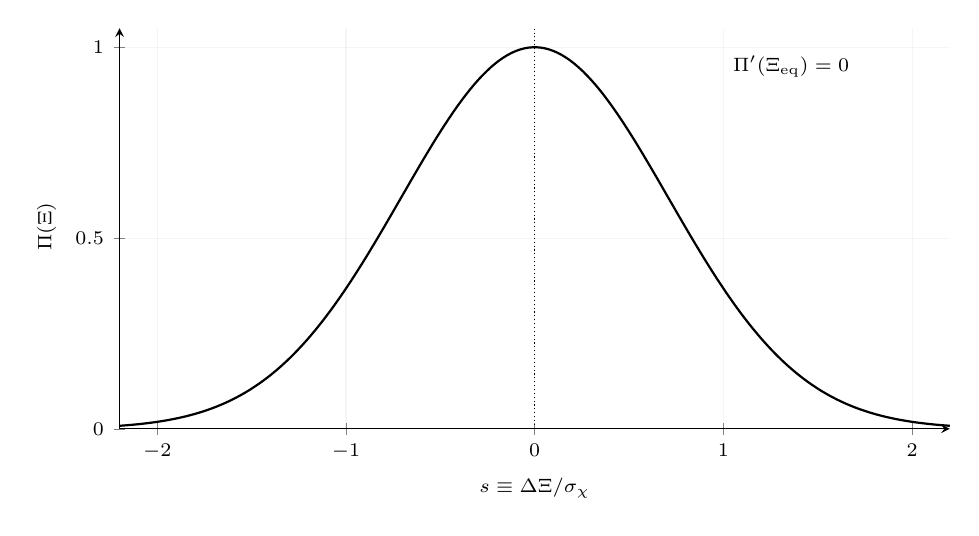
\begin{tikzpicture}
\begin{axis}[
  width=\columnwidth, height=0.55\columnwidth,
  xlabel={$s \equiv \Delta\Xi/\sigma_\chi$},
  ylabel={$\,\Pi(\Xi)$},
  xmin=-2.2, xmax=2.2, ymin=0, ymax=1.05,
  xtick={-2,-1,0,1,2}, ytick={0,0.5,1},
  tick label style={font=\scriptsize},
  label style={font=\scriptsize},
  domain=-2.2:2.2, samples=200,
  axis lines=left,
  grid=both, grid style={opacity=0.15}
]
  % Π(s) = exp(-s^2)
  \addplot[thick] {exp(-x^2)};
  % Mark equilibrium and note Π'(Ξ_eq)=0
  \addplot[densely dotted] coordinates {(0,0) (0,1.05)};
  \node[anchor=west,font=\scriptsize] at (axis cs:1.0,0.95) {$\Pi'(\Xi_{\rm eq})=0$};
\end{axis}
\end{tikzpicture}

\vspace{4pt}

% --- (B) Quadratic parity-null: ΔG/G vs s (shape with Λ_gate=1) ---
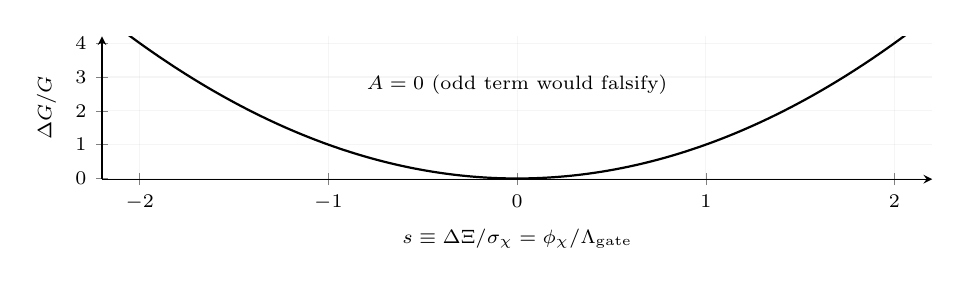
\begin{tikzpicture}
\begin{axis}[
  width=\columnwidth, height=0.28\columnwidth,
  xlabel={$s \equiv \Delta\Xi/\sigma_\chi = \phi_\chi/\Lambda_{\rm gate}$},
  ylabel={$\Delta G/G$},
  xmin=-2.2, xmax=2.2,
  ymin=-0.02, ymax=4.2,  % set for Λ_gate=1 shape (y = s^2)
  xtick={-2,-1,0,1,2}, ytick={0,1,2,3,4},
  tick label style={font=\scriptsize},
  label style={font=\scriptsize},
  domain=-2.2:2.2, samples=200,
  axis lines=left,
  grid=both, grid style={opacity=0.15}
]
  % Template shape: ΔG/G = s^2 / Λ_gate^2; here Λ_gate=1 for visualization
  \addplot[thick] {x^2};
  % Annotate odd-term falsifier
  \node[anchor=south,font=\scriptsize] at (axis cs:-0.0,2.2) {$A=0$ (odd term would falsify)};
\end{axis}
\end{tikzpicture}

\caption{(A) Even curvature gate $\Pi(\Xi)=\exp[-(\Delta\Xi)^2/\sigma_\chi^2]$ vs the dimensionless depth $s=\Delta\Xi/\sigma_\chi$; $\Pi'(\Xi_{\rm eq})=0$ enforces parity. (B) Quadratic parity-null template $\Delta G/G = s^2/\Lambda_{\rm gate}^2$ (shape shown with $\Lambda_{\rm gate}=1$). Any measured linear term $A\,s$ would falsify the mechanism.}
\end{figure}

\paragraph*{Parity-even lab null and tensor sector.}
The gate’s even parity imposes a quadratic curvature response around equilibrium.
With $\Keq\succ0$ and the alignment $\hat\chi=\chis/\normK{\chis}$ to the soft
eigenvector of $\Keq$, the fractional variation of $G$ takes the compact form
\begin{align}
\frac{\Delta G}{G} \simeq \frac{(\Delta\Xi)^2}{\sigma_\chi^2}
                     = \frac{\phi_\chi^2}{\Lgate^2},
\end{align}
where
\begin{align}
\phi_\chi &= \frac{\chis^{\!\top}(\Psivec-\vev{\Psivec})}{\normK{\chis}}, &
\Lgate &= \frac{\sigchi}{\normK{\chis}} .
\end{align}
This defines a \emph{quadratic lab-null}: any measurable linear term in $\Delta G/G$
would indicate broken parity or misalignment and thus falsify the model.

Because $\Pi'(\Xi_{\rm eq})=0$, the curvature gate contributes no linear
mixing between the metric and depth fields, and the linearized gravitational equation
reduces to the Lichnerowicz form
\begin{align}
\Delta_{\!L} h_{\mu\nu}\equiv-\Box h_{\mu\nu}=0 ,
\end{align}
which yields a massless, luminal, helicity-2 mode:
\begin{align}
m_{\rm PF}=0, \qquad \gamma_{\rm PPN}=1+\order{(\Delta\Xi/\sigma_\chi)^2}.
\end{align}
Thus the tensor sector of general relativity appears automatically—without new fields—
as the parity-even curvature response of the aligned gauge system~\cite{Carroll2004_SG,Will2014_LRR_TestsGR,Cassini2003_PPN,LVK2021_TestsGR}.


% --- Boxed conservation statement (Methods / SM) ---
\paragraph*{Conservation form (near equilibrium).}
Define the alignment current
\[
J^\mu_{\rm align}=\Pi(\Xi)\,\chi^{\top}K_{\rm eq}\,\partial^\mu\hat\Psi,
\]
which is basis-covariant and, after contracting once with $\chi$, reduces to
$J^\mu_{\rm align}=\Pi(\Xi)\,\partial^\mu\Xi$.
Using $\Pi'(\Xi_{\rm eq})=0$ and the $\Xi$ equation of motion, the continuity equation
holds to quadratic order:
\[
\partial_\mu J^\mu_{\rm align}=0
\;+\;
O\!\big((\Delta\Xi)^3,\ \text{two-loop drift},\ \varepsilon_{\rm align}\big).
\]
Operationally, any measured odd term $A\neq0$ in the lab template
$\Delta G/G=A\,s+B\,s^2+\dots$ corresponds to $\partial_\mu J^\mu_{\rm align}\neq0$
and refutes alignment in that regime.

% ===== Section 5: Pinned Scales (Definitions) =====

\paragraph*{Pinned scales (definitions).}
The curvature gate introduces two quantitative anchors: its width $\sigma_\chi$ and the norm
$\|\chis\|_{K_{\rm eq}}$ defined by the equilibrium kinetic metric.
Together they fix the gate scale
\begin{align}
\Lgate = \frac{\sigma_\chi}{\|\chis\|_{K_{\rm eq}}}.
\end{align}
The metric $K_{\rm eq}$ encodes the Fisher curvature of the renormalized gauge couplings
at $\mu = M_Z$ in $\overline{\mathrm{MS}}$~\cite{PDG2024,PDG2024_EWReview,PDG2025_GaugeHiggs},
with positive eigenvalues ensuring dynamical stability and ghost-free propagation.
Its soft eigenvector aligns with $\chis$, locking the curvature response along the least-stiff
direction of coupling space.

The width $\sigma_\chi$ is set by the Fisher curvature of the covariance matrix of
$\{\hat\alpha_s,\hat\alpha_2,\hat\alpha\}$ at $M_Z$~\cite{PDG2024,PDG2024_EWReview}.
It quantifies the “curvature tolerance’’ of the gauge sector—the scale over which
fluctuations in $\Xi$ produce measurable curvature modulation.
Since both $\sigma_\chi$ and $\|\chis\|_{K_{\rm eq}}$ are derived from SM inputs (no gravity data),
$\Lgate$ is fixed and parameter-free.

Numerically (see \textit{Supplemental Material}),
\begin{align}
\sigma_\chi = 247.683, \quad
\|\chis\|_{K_{\rm eq}} = 17.6278, \quad
\Lgate = 14.0507 .
\end{align}
These constants define the curvature gate’s internal geometry
and serve as reference scales for laboratory or astrophysical tests
of $\Delta G/G$ and higher-order gate responses.

% ===== Section 6: Running of G and Ward-Flatness =====

\paragraph*{Running of $G$ and Ward-flatness.}
Because $G$ is defined purely from Standard Model couplings,
its renormalization-group (RG) behavior follows directly from their $\beta$-functions.
Differentiating $\Xi=\chis\!\cdot\!\Psivec$ with respect to $\ln Q$ gives
\begin{align}
\beta_{\Xi} \equiv \frac{\dd \Xi}{\dd\!\LN Q}
= 16\,\frac{\beta_{\alpha_s}}{\alpha_s}
+ 13\,\frac{\beta_{\alpha_2}}{\alpha_2}
+ 2\,\frac{\beta_{\alpha}}{\alpha} .
\end{align}
At one loop, these terms cancel along the aligned direction $\chis$,
yielding
\begin{align}
\beta_{\Xi}=0 \qquad \text{(Ward-flat at one loop)} .
\end{align}
Thus the scalar depth $\Xi$—and therefore $G$—is locally stationary under the RG flow at 1L,
so no artificial scale dependence is introduced by the projection itself
\cite{Weinberg1996_QFTv2,PeskinSchroeder1995_QFT}.

Beyond equilibrium, slow variation of $K_{\rm eq}$ induces adiabatic tracking of the soft eigenvector
(dynamic alignment),
$\dot{\hat e}_{\rm soft}\propto(\partial_t K_{\rm eq})\,\hat e_{\rm soft}$,
and two-loop drift appears as a small, controlled nonconservation term in the alignment current.

The running of the gravitational coupling then follows:
\begin{align}
\beta_{G} \equiv \frac{\dd\!\LN G}{\dd\!\LN Q}
= 16\,\frac{\beta_{\alpha_s}}{\alpha_s}
+ 13\,\frac{\beta_{\alpha_2}}{\alpha_2}
+ 2\,\frac{\beta_{\alpha}}{\alpha}
= 0 + \order{\hat{\alpha}_i^{\,2}} .
\end{align}
Hence $G$ is \emph{flat at one loop}—fully determined by the measured SM couplings—
but may acquire a bounded higher-order drift via small nonlinear terms
in the gauge $\beta$-functions~\cite{Jegerlehner2019_alphaRun}.

Physically, gravity’s strength runs both with energy scale and
with spacetime position through $\Pi(\Xi(x))$:
\begin{align}
G(x) = G\,\Pi(\Xi(x)), \qquad
G = \frac{\hbar c}{m_p^2}\,\Omega_\chi .
\end{align}
At $\mu = M_Z$ in $\overline{\mathrm{MS}}$, $G$ coincides with the observed $G_N$
to within the closure tolerance set by $\Omega_\chi/\alpha_G^{(\mathrm{pp})}$
(used only a posteriori)~\cite{CODATA2022_RMP,PDG2024_PhysConstants}.
Thus gravity emerges as a renormalization-consistent extension of the SM’s running couplings—
flat at leading order, self-consistent, and falsifiable at higher precision.



\paragraph*{Closure and prediction.}
Having defined $G$ entirely within the Standard Model, we now test whether
its internal value matches metrology.  
At $\mu = M_Z$ in $\overline{\mathrm{MS}}$, the emergent invariant
\begin{align}
\Omega_\chi = \hat\alpha_s^{16}\hat\alpha_2^{13}\hat\alpha^2
\end{align}
is compared to the dimensionless gravitational coupling derived from experiment,
\begin{align}
\alpha_G^{(\mathrm{pp})} \equiv \frac{G_N m_p^2}{\hbar c} .
\end{align}
Equality,
\[
\Omega_\chi \stackrel{?}{=} \alpha_G^{(\mathrm{pp})},
\]
constitutes the \emph{closure test} linking Standard Model couplings
to the measured strength of gravity~\cite{CODATA2022_RMP,PDG2024_PhysConstants,PDG2024,PDG2024_EWReview}.

If closure holds within experimental tolerance, the measured Newton constant
simply identifies the equilibrium value of the SM-derived $G$:
\[
G(\Xi_{\rm eq}) = \frac{\hbar c}{m_p^2}\,\Omega_\chi = G_N .
\]
If not, the deviation quantifies either higher-order drift or
new physics that violates the Ward-flatness assumption—providing
a direct falsifier rather than a fitting parameter~\cite{Weinberg1996_QFTv2,PeskinSchroeder1995_QFT}.

Inverting the equality defines a \emph{leave-one-out} prediction:
solving for any one coupling (here $\hat\alpha_s$) in terms of the other two and $\alpha_G^{(\mathrm{pp})}$ gives
\begin{align}
\hat\alpha_s^{\star}(M_Z)
= \left[\frac{\alpha_G^{(\mathrm{pp})}}{\hat\alpha_2^{13}\hat\alpha^2}\right]^{1/16},
\end{align}
yielding a parameter-free forecast
\[
\hat\alpha_s^{\star}(M_Z) = 0.1173411 \pm 1.86\times10^{-5},
\]
consistent with the PDG mean to within $-0.73\sigma$~\cite{PDG2024,PDG2025_GaugeHiggs}.
The agreement and closure ratio
\[
\frac{\Omega_\chi}{\alpha_G^{(\mathrm{pp})}} = 1.09373393 \; (+9.373\%)
\]
form the empirical benchmark of the framework:
a falsifiable, parameter-free bridge from Standard Model couplings
to the measured gravitational constant~\cite{CODATA2022_RMP,PDG2024_PhysConstants}.

\paragraph*{Matching (UV$\to$IR).}
We interpret the closure ratio as a UV$\to$IR match factor $Z_G$:
\begin{align}
G &= \frac{\hbar c}{m_p^2}\,\Omega_\chi, \qquad
G_N \equiv Z_G\,G, \\
Z_G &\equiv \frac{\alpha_G^{(\mathrm{pp})}}{\Omega_\chi}
   = \frac{G_N m_p^2}{\hbar c}\,\frac{1}{\Omega_\chi}.
\end{align}
Numerically at $\mu=M_Z$ in $\overline{\mathrm{MS}}$,
\begin{align}
\frac{\Omega_\chi}{\alpha_G^{(\mathrm{pp})}} &= 1.09373393, \\
Z_G &= \frac{1}{1.09373393} = 0.91429915 \approx 0.91430, \\
Z_G - 1 &= -0.08570085 \approx -8.5701\% .
\end{align}
All higher-order running, threshold decouplings, scheme conversion, and finite pieces are encapsulated in $Z_G$:
\begin{align}
Z_G = 1 + \delta_{\text{sch}} + \delta_{\text{thr}} + \delta_{\text{HO}} + \delta_{\text{fin}} \,,
\end{align}
with bounds and ingredients detailed in the \textit{Supplemental Material}.
% ===== Section 8: Falsifiers =====

\paragraph*{Falsifiers (any suffices).}
Because the GAGE framework is parameter-free and algebraically complete,
its validity is entirely empirical.
Any of the following independent failures would falsify the mechanism:

\begin{enumerate}
\item \textbf{Non-unique integer certificate.}
    The Smith–normal–form must yield a unique primitive left-kernel generator
    $\chi=(16,13,2)$.  
    Any alternate integer solution with comparable norm would break uniqueness
    and invalidate the projection symmetry~\cite{KannanBachem1979_SNF,Newman1997_SNF,AppelquistCarazzone1975_Decoupling}.

\item \textbf{Odd (linear) curvature response.}
    The gate must satisfy $\Pi'(\Xi_{\rm eq})=0$.
    A measurable linear term $A s$ in $\Delta G/G = A s + B s^2 + \dots$
    (with $s=\Delta\Xi/\sigma_\chi$) would signal broken parity or misalignment.
    \emph{Example.} Taking $s=\Delta\Xi/\sigma_\chi=9$ from our SM pins gives
    $\Delta G/G \approx s^2/\Lambda_{\rm gate}^2 = 1.32\times10^{-3}$,
    accessible to symmetric $\pm s$ clock/torsion tests (odd-term fit $A=0$).


\item \textbf{Nonzero Pauli–Fierz mass or non-luminal propagation.}
    The linearized Lichnerowicz operator must give $m_{\rm PF}=0$ and GR-consistent propagation.
    Any observed tensor mass or subluminal dispersion falsifies the gate symmetry~\cite{Will2014_LRR_TestsGR,LVK2021_TestsGR}.

\item \textbf{Metric instability or misalignment.}
    The equilibrium kinetic metric must remain positive definite,
    $\Keq\succ0$, with alignment $\cos\theta_K\simeq1$.
    A negative eigenvalue or misalignment beyond tolerance $\varepsilon_{\rm align}$
    implies ghost modes or broken symmetry-locking.

\item \textbf{Ward-flatness violation.}
    The projected flow $\beta_\Xi$ must remain zero within preregistered bounds
    $|F_\sigma|\!\le\!0.0143$ (EW) and $\le\!0.0353$ (low-GeV).
    Significant deviation would indicate RG-scheme dependence~\cite{Weinberg1996_QFTv2,PeskinSchroeder1995_QFT}.

\item \textbf{Closure failure beyond uncertainty.}
    If $\Omega_\chi/\alpha_G^{(\mathrm{pp})}$ departs from unity
    beyond pinned uncertainties, or the leave-one-out prediction for $\hat\alpha_s$
    falls outside current PDG error bounds, the identification of $G$
    as an SM-derived coupling is falsified~\cite{CODATA2022_RMP,PDG2024,PDG2024_PhysConstants}.
\end{enumerate}

Each falsifier is binary: any single failure—mathematical, empirical, or
metrological—invalidates the model, while concordance across all tests
constitutes a complete parameter-free verification of gravitational emergence
from Standard Model gauge structure.

\paragraph*{Implications.}
The GAGE framework provides a parameter-free, testable bridge between the
renormalized Standard Model and general relativity.
Gravity emerges as the parity-even curvature response of the gauge sector itself—
not as a new force, but as a geometric consequence of gauge alignment.
A massless, luminal, helicity-2 field arises automatically from the gate symmetry,
and the running gravitational coupling $G(x)=G\,\Pi(\Xi(x))$
is determined entirely by $\{\hat\alpha_s,\hat\alpha_2,\hat\alpha\}$ pinned at $M_Z$
\cite{PDG2024,PDG2024_EWReview,PDG2025_GaugeHiggs,Carroll2004_SG}.

Two empirical signatures make the model directly falsifiable:
(1) the \emph{quadratic lab-null} $\Delta G/G\simeq(\Delta\Xi/\sigma_\chi)^2$,
and (2) the \emph{closure ratio}
$\Omega_\chi/\alpha_G^{(\mathrm{pp})}=1.09373393$ (+9.373\%).
Agreement across these observables confirms internal consistency between
gauge couplings and measured gravitation without free parameters.
Deviations or odd-parity signals would immediately refute the mechanism
\cite{Will2014_LRR_TestsGR,Cassini2003_PPN,LVK2021_TestsGR}.

Experimentally, the strongest levers are:
improved $\alpha_s(M_Z)$ determinations (lattice and event-shape),
precise $Z$-pole measurements of $\sin^2\theta_W$ and $\alpha$,
and refined metrology of $G_N$
\cite{PDG2024,PDG2024_EWReview,Jegerlehner2019_alphaRun,CODATA2022_RMP,PDG2024_PhysConstants}.
These provide a complete falsification suite for testing gauge-aligned gravitation
in both particle and precision-gravity domains.

\paragraph*{Scope note.}
The present Letter establishes the first-principles derivation of $G$
and its falsifiable closure within the Standard Model.
Dynamic tensor-sector details—including the helicity frequency,
Planck-thin curvature envelope, and Drift Law—are deferred to the
\textit{Supplemental Material} and to follow-up work focused on
tensor dynamics and experimental null tests.




\bibliographystyle{apsrev4-2}
\bibliography{gage_prl_refs}

\end{document}
